\documentclass[../../main.tex]{subfiles}

\begin{document}

La metodología a usar en este presente proyecto es la metodología Agile, ya que es una de las más usadas actualmente en el sector del desarrollo que permite dar un enfoque iterativo en el que evaluar de forma constante los resultados.
Bajo esta metodología se hará uso del método Scrum, la cual se utiliza para desarrollar y abordar problemas complejos de
una manera eficiente y sencilla.

\begin{figure}[h]
\centering
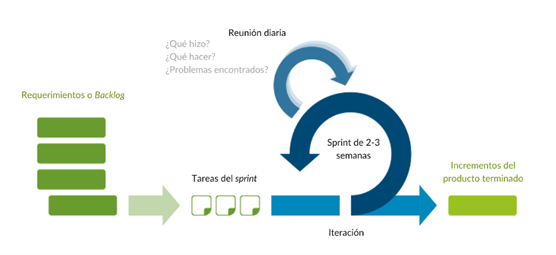
\includegraphics[width=\textwidth]{images/1_introduccion/scrum.png}
\caption{Metodología SCRUM}
\end{figure}

Por como funciona el proceso Scrum es el motivo por el cual se implementa en este proyecto, dado que se ejecutan ciclos de intervalos cortos de 2 a 4 semanas en la cual en cada iteración es preciso proporcionar un resultado completo, consiguiendo que finalmente se incremente de forma iterativa el producto final con el mínimo esfuerzo cuando el cliente lo solicite.

En este proyecto los roles con el método Scrum serían los siguientes:
\begin{itemize}
    \item \textbf{Scrum Master}: Es el responsable de que las técnicas Scrum sean comprendidas y aplicadas en la organización. Es el mánager de Scrum, un líder que se encarga de eliminar impedimentos o inconvenientes que tenga el equipo dentro de un sprint. Este rol será compartido entre el tutor y co-tutor del trabajo fin de grado, Ángel Mora y Domingo López Rodríguez.
    \item \textbf{Desarolladores}: Son los responsables de realizar y entregar el producto en cada sprint. En este rol el encargado es el presente autor del trabajo fin de grado, Jean-Paul Beaudry. 
\end{itemize}


\end{document}